\chapter{Protocols}

\clearpage
\section{Password Eavesdropping Risks}
A good case study comes from simple embedded systems, such as the remote control used to open
your garage or to unlock the doors of cars manufactured up to the mid-1990’s.
These primitive remote controls just broadcast their serial number, which also
acts as the password. An attack that became common was to use a ‘grabber’, a device 
that would record a code broadcast locally and replay it later. 

sixteen-bit passwords are too short. It occasionally happened that people found they could unlock 
the wrong car by mistake. By the mid-1990’s, devices appeared which could try all
possible codes one after the other. A code will be found on average after about
215 tries, which at ten per second takes under an hour. A thief operating in a
parking lot with a hundred vehicles within range would be rewarded in less
than a minute with a car helpfully flashing its lights.



\section{Simple Authentication}

	{\bf Nonce:} The term nonce can mean anything that guarantees the freshness of a
	message. A nonce can, according to the context, be a random number, a serial
	number, a random challenge received from a third party, or even a timestamp.

	{\bf Security and business: } Security mechanisms are used more and more to support business 
	models, by accessory control, rights management, product tying and bundling. It is
	wrong to assume blindly that security protocols exist to keep ‘bad’ guys ‘out’.
	They are increasingly used to constrain the lawful owner of the equipment in
	which they are built; their purpose may be of questionable legality or contrary
	to public policy. For example: Many printer companies embed authentication mechanisms 
	in printers to ensure that genuine toner cartridges are used. If a competitor’s 
	product is loaded instead, the printer may quietly downgrade from 1200 dpi to 300 dpi, 
	or simply refuse to work at all. Mobile phone vendors make a lot of money from 
	replacement batteries, and now use authentication protocols to spot competitors’ 
	products so they can be blocked or even drained more quickly. 

	\clearpage
	\subsection{Challenge and response}

		Many cars use a more sophisticated two-pass protocol, called challenge-response, 
		to actually authorise engine start. As the car key is inserted into the steering lock, 
		the engine controller sends a challenge consisting of a random n-bit number to the key 
		using short-range radio. The car key computes a response by encrypting the challenge. 
		This is still not bulletproof, how random is random?

		{\bf two-factor authentication:} A much more visible use of challenge-response is in two-factor authentication.
		Many organizations issue their staff with password generators to let them
		log on to corporate computer systems. These may look like calculators
		but their main function is as follows; when you want to log in to a machine on the network, 
		you call up a logon screen and are presented with a random challenge of maybe seven digits. 
		You key this into your password generator, together with a PIN of maybe four
		digits. The device encrypts these eleven digits using a secret key shared with
		the corporate security server, and displays the first seven digits of the result.
		You enter these seven digits as your password.

	\subsection{Reflection Attacks}
		--Write something here?--

\clearpage
\section{Manipulating the Message}

	An example is when dishonest cabbies insert pulse generators in the cable
	that connects their taximeter to a sensor in their taxi’s gearbox. The sensor
	sends pulses as the prop shaft turns, which lets the meter work out how far
	the taxi has gone. A pirate device, which inserts extra pulses, makes the taxi
	appear to have gone further. 

	Another example is a key log attack which defeated many pay-TV systems. 
	If the messages that pass between the smartcard and the decoder are the same for
	all decoders (which is usually the case) then a subscriber can log all the keys
	sent by his card to his decoder and post it online somewhere. People without a
	subscription, but who have video-recorded the enciphered program, can then
	download the key log and use it to decipher the tape.

	
\section{Changing the Environment}

	A very common cause of protocol failure is that the environment changes, so
	that assumptions which were originally true no longer hold and the security
	protocols cannot cope with the new threats.

	For example, a passenger who commuted a long distance from a suburban station 
	to downtown might buy two cheaper, short distance season tickets — one between 
	his suburban station and a nearby one, and the other between his destination 
	and another downtown station. 

	An other example is a one-day travel pass in London.
	When a one-day travel pass was sold, the revenue was distributed between 
	the various bus, train and subway operators using a formula that depended on where it 
	was sold. Suddenly, the train companies had a motive to book all their ticket sales 
	through the outlet that let them keep the largest percentage. As well as bad outsiders
	(passengers), we now had bad insiders (rail companies), and the design just
	hadn’t allowed for them. Chaos and litigation ensued.

	The transport system’s problem was not new; it had been observed in the
	Italian ski resort of Val di Fassa in the mid-1970’s. There, one could buy a
	monthly pass for all the ski lifts in the valley. An attendant at one of the lifts
	was observed with a deck of cards, one of which he swiped through the reader
	between each of the guests. It turned out that the revenue was divided up
	between the various lift operators according to the number of people who had
	passed their turnstiles. So each operator sought to inflate its own figures as
	much as it could.


\section{Chosen Protocol Attacks}
	Here’s one example. It used to be common for people visiting a porn
	website to be asked for ‘proof of age,’ which usually involves giving a
	credit card number, whether to the site itself or to an age checking service.
	If credit and debit cards become usable in PCs, it would be natural for
	the porn site to ask the customer to authenticate a random challenge as
	proof of age. A porn site can then mount a ‘Mafia-in-the-middle’ attack. 
	They wait until an unsuspecting customer visits their site,
	then order something resellable (such as gold coins) from a dealer, playing
	the role of the coin dealer’s customer. When the coin dealer sends them the
	transaction data for authentication, they relay it through their porn site to
	the waiting customer. The poor man OKs it, the Mafia gets the gold coins, and
	when thousands of people suddenly complain about the huge charges to their
	cards at the end of the month, the porn site has vanished — along with the
	gold. 


\section{Managing Encryption Keys}

	Authentication protocols are now also used in distributed computer systems
	for general key management purposes, and are therefore becoming ever more
	important. Kerberos was the first such system to come into widespread use,
	and a variant of it is used in Windows. 

	\subsection{Basic Key Management}
		The basic idea behind key distribution protocols is that where two princi-
		pals want to communicate, they may use a trusted third party to effect an
		introduction.
		When discussing authentication protocols, it is conventional to give the
		principals human names in order to avoid getting lost in too much algebraic
		notation. So we will call the two communicating principals {\bf ‘Alice’} and 
		{\bf ‘Bob’}, and the trusted third party {\bf ‘Sam’}. 

		A simple authentication protocol could run as follows.
		\begin{enumerate}
			\item Alice first calls Sam and asks for a key for communicating with Bob.
			\item Sam responds by sending Alice a pair of certificates. Each contains a copy
			of a key, the first encrypted so only Alice can read it, and the second
			encrypted so only Bob can read it.
			\item Alice then calls Bob and presents the second certificate as her introduction.
			Each of them decrypts the appropriate certificate under the key they share
			with Sam and thereby gets access to the new key. Alice can now use the
			key to send encrypted messages to Bob, and to receive messages from him
			in return.
		\end{enumerate}

		\begin{figure}[H]
			\centering
			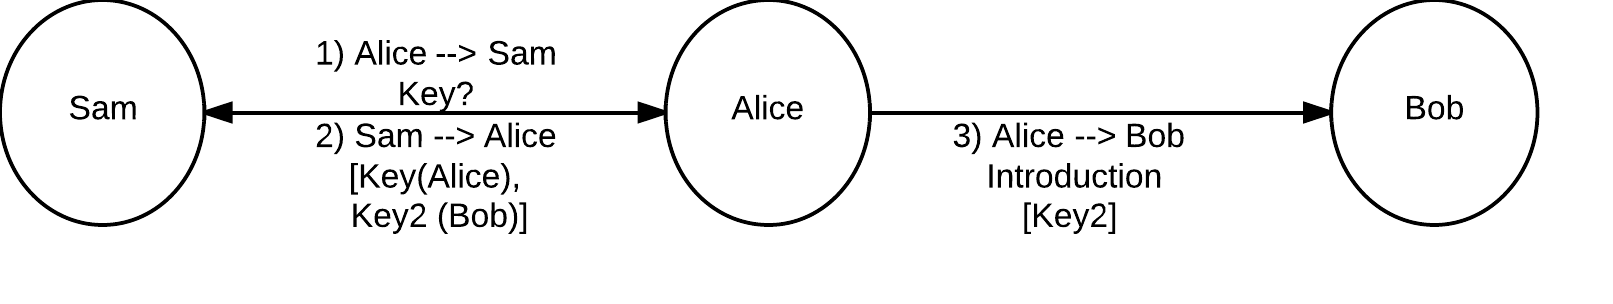
\includegraphics[scale=0.20]{pics/BobAliceSam1.png}
		\end{figure}

		Expanding the notation, Alice calls Sam and says she’d like to talk to
		Bob. Sam makes up a session key message consisting of Alice’s name, Bob’s
		name, a key for them to use, and a timestamp. He encrypts all this under
		the key he shares with Alice, and he encrypts another copy of it under the
		key he shares with Bob. He gives both ciphertexts to Alice. Alice retrieves
		the key from the ciphertext that was encrypted to her, and passes on to
		Bob the ciphertext encrypted for him. She now sends him whatever message
		she wanted to send, encrypted using this key.
		Replay attacks are a known problem with authentication protocols, so in
		order that both Bob and Alice can check that the certificates are fresh, Sam may
		include a timestamp in each of them. If certificates never expire, there might
		be serious problems dealing with users whose privileges have been revoked.

		\begin{figure}[H]
			\centering
			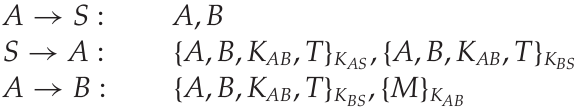
\includegraphics[scale=0.5]{pics/basicKeyManagement.png}
		\end{figure}

	\subsection{The Needham-Schroeder Protocol}
		Many existing key distribution protocols are derived from the Needham-Schroeder
		protocol, which appeared in 1978 [960]. It is somewhat similar to the above,
		but uses nonces rather than timestamps. It runs as follows:

		\begin{figure}[H]
			\centering
			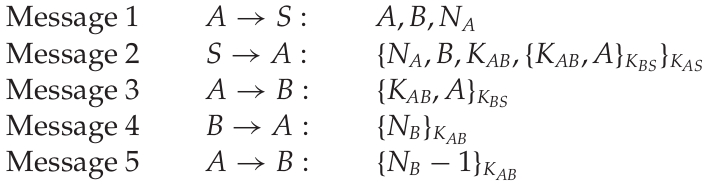
\includegraphics[scale=0.4]{pics/NeedhamSchroederProtocol.png}
		\end{figure}

		Here Alice takes the initiative, and tells Sam: ‘I’m Alice, I want to talk to Bob,
		and my random nonce is NA .’ Sam provides her with a session key, encrypted
		using the key she shares with him. This ciphertext also contains her nonce so
		she can confirm it’s not a replay. He also gives her a certificate to convey this
		key to Bob. She passes it to Bob, who then does a challenge-response to check
		that she is present and alert.

		There is a subtle problem with this protocol — Bob has to assume that the
		key KAB he receives from Sam (via Alice) is fresh. This is not necessarily so.

	\subsection{Kerberos}
		An important practical derivative of the Needham-Schroeder protocol may be
		found in Kerberos, a distributed access control system that originated at MIT
		and is now one of the standard authentication tools in Windows. Instead
		of a single trusted third party, Kerberos has two kinds: an authentication server
		to which users log on, and a ticket granting server which gives them tickets
		allowing access to various resources such as files. This enables more scalable
		access management. In a university, for example, one might manage students
		through their halls of residence but manage file servers by departments; in
		a company, the personnel people might register users to the payroll system
		while departmental administrators manage resources such as servers and
		printers.

		\begin{figure}[H]
			\centering
			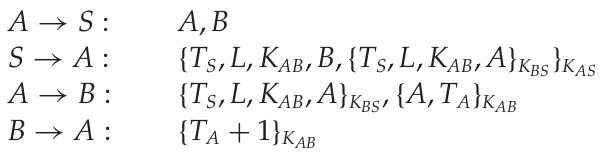
\includegraphics[scale=0.5]{pics/Kerberos.png}
		\end{figure}
		
		Translating this into English: Alice asks the ticket granting server for access
		to B. If this is permissible, the ticket {TS , L, KAB , A}KBS is created containing a
		suitable key KAB and given to Alice to use. She also gets a copy of the key
		in a form readable by her, namely encrypted under KAS . She now verifies the
		ticket by sending a timestamp TA to the resource, which confirms it’s alive by
		sending back the timestamp incremented by one (this shows it was able to
		decrypt the ticket correctly and extract the key KAB ).
		The vulnerability of Needham-Schroeder has been fixed by introducing
		timestamps rather than random nonces. But, as in most of life, we get little
		in security for free. There is now a new vulnerability, namely that the clocks
		on our various clients and servers might get out of synch; they might even be
		desynchronized deliberately as part of a more complex attack.

\section{Getting Formal}

	There are a number of different approaches to verifying the correctness
	of protocols. The best known is the logic of belief, or BAN logic. 
	It reasons about what a principal might reasonably believe having seen 
	of certain messages, time-	stamps and so on. A second is the random oracle 
	model, which is described in the chapter on cryptology and which is favored 
	by people working on the theory of cryptography.
	Finally, a number of researchers have applied mainstream formal methods
	such as CSP and verification tools such as Isabelle.

	\subsection{The BAN Logic}

	\begin{figure}[H]
		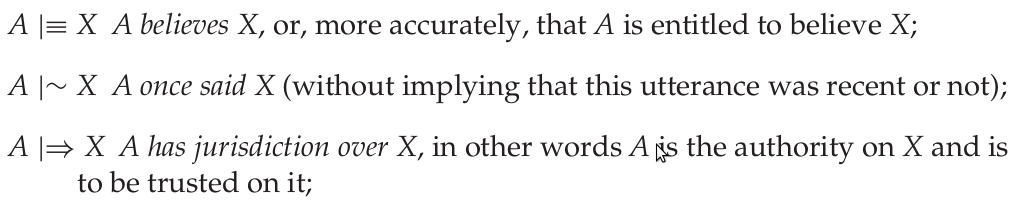
\includegraphics[scale=0.3]{pics/BAN1.png}
	\end{figure}
	\begin{figure}[H]
		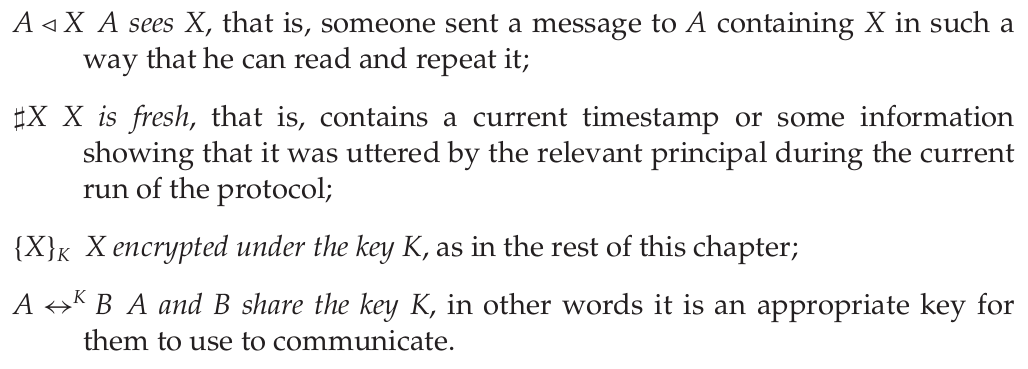
\includegraphics[scale=0.3]{pics/BAN2.png}
	\end{figure}
	\begin{figure}[H]
		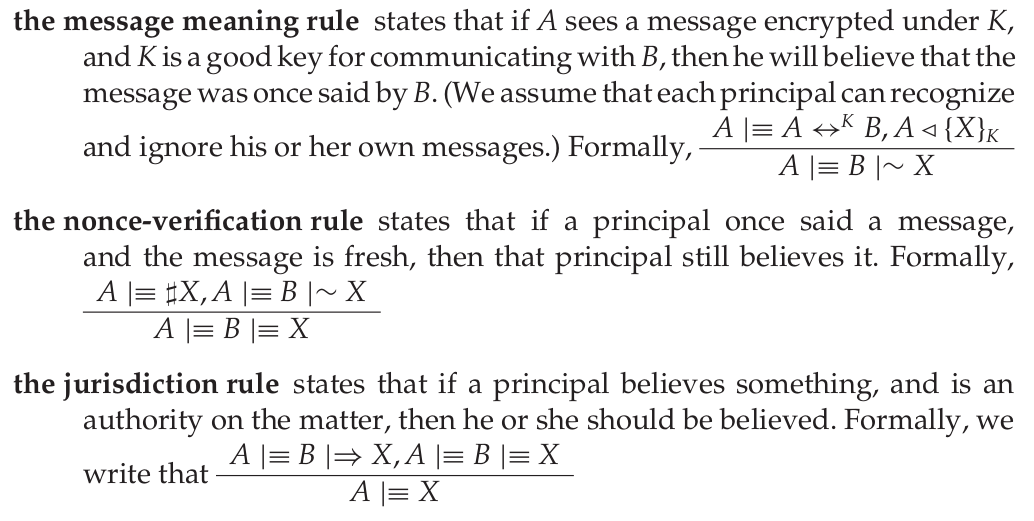
\includegraphics[scale=0.3]{pics/BAN3.png}
	\end{figure}



